\documentclass[11pt]{article}
\usepackage[T1]{fontenc}
\usepackage{lmodern,microtype}
\usepackage[a4paper,margin=27mm]{geometry}
\usepackage{amsmath,amssymb,amsthm,mathtools,booktabs}
\usepackage[dvipsnames]{xcolor}
\usepackage{tikz}
\usepackage[hidelinks]{hyperref}
\usepackage[nameinlink,noabbrev]{cleveref}
\hypersetup{pdftitle={Physical Gluing and Wilson Constraints from Euclidean Tensor Prices},pdfauthor={}}
\setlength{\parskip}{0.15em}
\setlength{\emergencystretch}{1.8em}
\numberwithin{equation}{section}
\newtheorem{theorem}{Theorem}[section]
\newtheorem{proposition}[theorem]{Proposition}
\newtheorem{lemma}[theorem]{Lemma}
\newtheorem{corollary}[theorem]{Corollary}
\theoremstyle{definition}
\newtheorem{definition}[theorem]{Definition}
\theoremstyle{remark}
\newtheorem{remark}[theorem]{Remark}
\DeclareMathOperator{\Hom}{Hom}
\DeclareMathOperator{\rank}{rank}
\DeclareMathOperator{\Tr}{Tr}
\newcommand{\Id}{\mathbf{1}}
\newcommand{\Cat}{\mathcal C}
\newcommand{\Center}{\mathcal Z}
\newcommand{\State}{\mathcal V}
\newcommand{\su}{\mathrm{SU}(2)_k}
\newcommand{\FF}{\mathbb C}
\title{\bfseries Physical Gluing and Wilson Constraints\\[-1pt] from Euclidean Tensor Prices}
\author{}
\date{}
\begin{document}
\maketitle
\vspace{-1.2em}
\begin{abstract}
We apply compatible Euclidean tensor prices to the physical cylinders of a unitary Turaev--Viro theory. Pricing the Choi tensors of charge-filtered cylinders gives the ranks after the physical constraint projector has been imposed. In a positive reservoir of fusion charges, ratios of these finite ranks converge to intrinsic quantum dimensions and yield an associative probability law for marked sewing. For doubled \(\su\), diagonal fundamental defects generate a parity-matched sector, not just diagonal charges; the first finite deficit from the untruncated vacuum rank recovers \(k\). Coherent linear combinations of ordered charge-filter insertions give a different kind of invariant: a pencil has vanishing Choi tensor at the signed cycle coefficient of two recoupling bases. An actual level-two doubled four-puncture cylinder has such a zero at \(-1/16\). For arbitrary fusion multiplicities, a finite family of word pencils determines the simultaneous unitary equivalence class of the marked cuts. On the compact quantum torus, the ranks of a joint Wilson penalty recover the full marked character variety, including its degenerate points, and its Haar state count. The constructions use the established state-sum, recoupling, and Wilson operators as inputs.
\end{abstract}

\section{Introduction}

Turaev--Viro (TV) state sums give topological amplitudes and physical state spaces from a spherical fusion category \cite{TuraevViro,BalsamKirillov,BalsamII,BalsamIII}. A discretized cylinder generally projects onto a proper subspace of its kinematical boundary space. Consequently an invariant of the unprojected boundary factors need not be an invariant of the physical cylinder. In this paper we use the cylinder's physical input--output tensor, and place its two boundary terminals at specified sites for the Euclidean tensor price of \cite{OpenAIPrice}. The construction does not place individual lattice links at spatial points or assume that a gravitational Hilbert space factorizes across a spatial cut.

For a linear map \(A\), the two-terminal Euclidean price of its Choi tensor is a prescribed distance times \(\log_2\rank A\). This part of the price theorem agrees with ordinary matrix rank. The distinction in the applications below is which physical linear map is priced. An identity cylinder gives the physical rank. A charge-filtered cylinder records which part of that rank survives a sewing condition. A \emph{coherent pencil} combines alternative ordered sewings before the rank is evaluated, so that its rank drops upon exact cancellation. A nonzero scalar multiplying an isolated cylinder cannot be recovered by prices of that cylinder alone.

We give two boundary constructions for physical gluing and one for the classical space of allowed flat data. First, a reservoir of physical charge sectors produces intrinsic quantum dimensions and normalized fusion weights as limits of differences of logarithmic cylinder ranks. On the gravity-related compact \(\su\) state sum this records both a failure of diagonal-charge closure and the finite truncation wall. Second, prices of coherent cylinder pencils recover recoupling between marked cuts. The phases are fixed only relative to a coherent reference and within the usual freedom of choosing bases in channel blocks. Third, a joint penalty for three noncommuting torus Wilson operators has a large-level rank support equal to the marked compact character variety. Its normalized rank also recovers the Haar volume of the corresponding classical constraint region. None of the constructions assumes a new tensor spectral point beyond \cite{OpenAIPrice}. The approach uses known TV factorization, Frobenius--Perron dimensions, quantum \(\{6j\}\) data, and the separation of finite matrix tuples by traces of words \cite{EtingofNikshychOstrik,KauffmanLins,Procesi}. The contribution is to realize the corresponding tests on ordinary placed tensors made from physical topological operations.

\section{Physical cylinders and priced sewing}\label{sec:cylinder}

Let \(\Cat\) be a unitary spherical fusion category and set \(\Center=Z(\Cat)\). The simple center charges form a finite set \(I\), with vacuum \(0\). We use the extended TV formulation in which framed ribbon defects are labeled by center objects; equivalently we use the Reshetikhin--Turaev description for \(\Center\) \cite{BalsamKirillov,BalsamII,BalsamIII,MugerDouble}. On a sphere with ordered incoming charges \(X_1,\ldots,X_n\) and one outgoing charge \(b\), the physical state space is
\begin{equation}\label{eq:physical}
  \State_b(X_1,\ldots,X_n)
  =\Hom_{\Center}\bigl(b,X_1\otimes\cdots\otimes X_n\bigr).
\end{equation}
A reducible external label means the corresponding direct sum of physical sectors. On the image of the normalized cylinder projector, the cylinder acts as the identity. If the theta or trivalent bases are changed, one uses the induced unitary map on this image. This fixes the Hilbert and adjoint conventions for the priced operators. The interpretation of the compact \(\su\) model as related to Euclidean \(2+1\) gravity is the standard one of \cite{MizoguchiTada}; none of the proofs requires identifying a price with a space-time length or taking a gravitational semiclassical limit.

For finite Hilbert spaces \(H_{\rm in}\) and \(H_{\rm out}\) and a linear map \(A:H_{\rm in}\to H_{\rm out}\), write
\begin{equation}\label{eq:choi}
 \Xi(A)=\sum_s (Ae_s)\otimes\bar e_s
       \in H_{\rm out}\otimes\overline{H_{\rm in}},
 \qquad
 \mathsf h_L(A)=L\log_2\rank A ,
\end{equation}
where \(e_s\) is an orthonormal basis of \(H_{\rm in}\), \(L>0\) is the distance between the two receiver sites, and \(\log_2 0=-\infty\). The tensor in \eqref{eq:choi} is basis-independent. Matrix equivalence reduces it to the shared-label tensor of order \(\rank A\), so \(\mathsf h_L\) is exactly its price in the system of \cite[Thm.~1.1]{OpenAIPrice}. For brevity, define the normalized price value
\begin{equation}\label{eq:normalized}
     \mathsf f_L(A)=2^{\mathsf h_L(A)/L}=\rank A .
\end{equation}
Block direct sums add these values; tensor products multiply them. In particular, \(\Xi(A\oplus B)\) is a block direct sum at the two sites. Sewing operators \(A\) and \(B\) means forming the ordinary composition \(BA\), not taking a block direct sum or adding log prices.

The two terminals in \eqref{eq:choi} are the whole incoming and outgoing surface. If additional receivers copy one chosen orthonormal diagonal record of a projector of rank \(r\), the resulting tensor is \(\Delta_S(r)\), of forced price \(W(S)\log_2 r\) on receiver set \(S\) of mean width \(W(S)\) \cite{OpenAIPrice}. Its price does not depend on the choice of record basis, since any such records are related by local invertible maps on the receivers. This optional operation copies an explicitly selected basis label rather than an arbitrary unknown quantum state. The constructions below require only the canonical, two-terminal Choi tensor.

An annular charge projector \(P_c\) is the cylinder with the central idempotent for simple charge \(c\) inserted on a specified separating collar. Intrinsic TV factorization gives an orthogonal direct sum over that charge. Thus the Choi tensor of the marked cylinder obeys \eqref{eq:choi} with the \emph{physical} block dimension. When a computational change of cut coordinates leaves the marked collar unchanged, the insertion and the cylinder are conjugated by the same unitary. Relative triangulation changes preserve these operators under the standard physical identifications. A different marked curve can define a noncommuting observable; its effect is addressed in \cref{sec:recoupling}.

\section{The fusion law from physical rank ratios}\label{sec:fusion}

Write \(N_{ai}^{c}=\dim\Hom(c,a\otimes i)\), and set \(N_a=(N_{ai}^{c})_{i,c}\). For an object \(X\) which is a finite direct sum of simples use the same convention by linearity. We choose the reservoir object \(R=\bigoplus_{a\in I}a\); a reservoir puncture is allowed to occupy precisely this direct sum of framed sectors. Positivity of quantum dimensions and rigidity yield
\begin{equation}\label{eq:pf}
  N_a d=d_a d,\qquad d^{\mathsf T}N_a=d_a d^{\mathsf T},
  \qquad N_a^{\mathsf T}=N_{a^*},\qquad d=(d_i)_{i\in I}.
\end{equation}
These are the standard dimension identities; the resulting limit of native prices is as follows.

\begin{theorem}[Physical fusion price]\label{thm:fusion}
Fix a simple terminal charge \(b\), a nonzero test object \(X\), and a two-terminal placement with distance \(L>0\). Then
\begin{equation}\label{eq:fusionlimit}
 \lim_{m\to\infty}
 \frac{\mathsf h_L(I_{\State_b(X,R^{\otimes m})})
       -\mathsf h_L(I_{\State_b(R^{\otimes m})})}{L}
   =\log_2 d_X .
\end{equation}
The result is independent of \(b\) and the association used when sewing the same marked surface. On simple charges the right-hand side is the unique real function \(p\) with \(p(0)=0\) obeying
\begin{equation}\label{eq:dimensionlaw}
  2^{p(a)+p(b)}=\sum_{c\in I}N_{ab}^{c}\,2^{p(c)} .
\end{equation}
\end{theorem}

\begin{proof}
The undeformed \(N_R=\sum_a N_a\) is symmetric by rigidity and \(R=R^*\). Each entry is positive: for \(i,c\), a simple summand \(a\) of \(c\otimes i^*\) gives \(N_{a i}^{c}>0\) by Frobenius reciprocity. Let \(D_{\Center}^2=\sum_i d_i^2\). By \eqref{eq:pf} and the Perron--Frobenius theorem,
\[
 d_R^{-m}N_R^m\longrightarrow
      \frac{d\,d^{\mathsf T}}{D_{\Center}^2},
 \qquad
 d_R=\sum_i d_i .
\]
The ranks at the two terminals before and after adding \(X\) are
\[
 q_m(0;b)=(N_R^m)_{0b},\qquad
 q_m(X;b)=(N_XN_R^m)_{0b}.
\]
With our row convention the product fuses the reservoir on the left of \(X\). The braiding identifies the resulting multiplicity with that in the stated order. This use of the braiding only identifies the ranks; it does not identify arbitrary ordered ribbon amplitudes. These ranks are nonzero for sufficiently large \(m\); they are the dimensions of \eqref{eq:physical} and hence independent of association. Their ratio tends to \(d_X\). The price limit follows by \eqref{eq:choi}. Tensor product and direct sum of the simple sectors give \(d_a d_b=\sum_c N_{ab}^{c}d_c\), which gives \eqref{eq:dimensionlaw}. Conversely, if \(x_c=2^{p(c)}>0\) satisfies that equation, then \(N_R x=(\sum_a x_a)x\). The positive Perron eigenvector of \(N_R\) is unique up to scale, and \(x_0=1\) fixes \(x=d\).
\end{proof}

\begin{proposition}[Marked fusion law]\label{prop:law}
Place two simple charges \(a,b\), \(m\) reservoir defects, and a fixed terminal charge \(z\) on the sphere. Let \(P_c\) be the filter on the circle enclosing just \(a,b\). For large enough \(m\) the normalized physical trace of this filter equals
\begin{equation}\label{eq:conditional}
 2^{[\mathsf h_L(P_c)-\mathsf h_L(I)]/L}
   =\frac{N_{ab}^{c}\,q_m(c;z)}{q_m(a\otimes b;z)}
   \longrightarrow \mathcal P(c\mid a,b)
   :=\frac{N_{ab}^{c}d_c}{d_a d_b}.
\end{equation}
The limiting joint law for all nested cuts of a fusion tree is the product of the local kernels \(\mathcal P\). Marginalizing intermediate charges yields the same outer charge law under either association of three leaves.
\end{proposition}

\begin{proof}
The range of \(P_c\) is
\[
 \Hom(c,a\otimes b)\otimes\Hom(z,c\otimes R^{\otimes m})
\]
by physical factorization. This gives the rank in \eqref{eq:conditional}; the normalized Hilbert trace of a projector is its rank divided by \(\dim\State_z\). The limit follows from the same Perron ratio as in \cref{thm:fusion}. For a fusion tree, the product of the elementary ranks gives the product of multiplicities times the final reservoir rank. In the limit, the \(d\)'s entering one node's denominator cancel those in its children's numerators, leaving the root dimension divided by the product of leaf dimensions. This gives the stated product law. Finally, the sum over internal channels gives the same multiplicity of the final irrep in the two associations by categorical associativity, with a common factor of dimensions.
\end{proof}

The trace state and the nested cut observables are specified in \cref{prop:law}. General states on a fixed block need not produce \(\mathcal P\), and the result does not assign a joint classical distribution to noncommuting crossing cuts. The reservoir does not supply any preassigned quantum dimension as a receiver coordinate. A finite integer rank ratio, not a categorical loop weight inserted by hand, is the quantity in \eqref{eq:fusionlimit}.

\section{Doubled \texorpdfstring{\(\su\)}{SU(2)k}: a closure test and a finite wall}\label{sec:closure}

For the compact input category \(\Cat=\su\), the center is \(\su\boxtimes\su^{\rm rev}\) \cite{MugerDouble}. Write \(f=1/2\), \(a=(f,f)\), and
\[
 \vartheta=\frac{\pi}{k+2},\qquad
 d^{\rm ch}_f=2\cos\vartheta,\qquad x=d_a=4\cos^2\vartheta .
\]
Here and below the chiral labels are spins \(0,1/2,\ldots,k/2\) with the unitary \(SU(2)\) fusion convention \cite{KauffmanLins}. Although the seed \(a\) has equal chiral labels, when \(k\ge2\) the two-seed fusion product includes four distinct channels. \Cref{prop:law} gives
\begin{center}
\begin{tabular}{c@{\quad}cccc}
\toprule
 \(c\) & \((0,0)\) & \((0,1)\) & \((1,0)\) & \((1,1)\)\\
 \(\mathcal P(c\mid a,a)\) &
 \(x^{-2}\) & \((x-1)x^{-2}\) & \((x-1)x^{-2}\) & \((x-1)^2x^{-2}\)\\
\bottomrule
\end{tabular}
\end{center}
The off-diagonal sectors therefore carry total limiting weight \(2(x-1)/x^2>0\). Discarding them changes the physical cylinder trace law.

\begin{proposition}[Minimal fusion-closed sector]\label{prop:closure}
For \(k\ge1\), the full fusion subcategory generated by \(a=(f,f)\) has simple labels
\begin{equation}\label{eq:parity}
  \mathcal D_{\rm simp}
     =\{(u,v):2u\equiv 2v \pmod 2\}.
\end{equation}
Its transparent subcategory is generated by the boson
\(J=(k/2,k/2)\) and is equivalent to \(\operatorname{Rep}(\mathbb Z_2)\).
\end{proposition}

\begin{proof}
In one chirality the fusion action of \(f\) is the adjacency matrix \(A_{k+1}\) of the path on twice-spin labels \(0,\ldots,k\). Every allowed target \(i\) is reached from \(0\) at all sufficiently large walk lengths congruent to \(i\) modulo two: start with the shortest walk and insert backtracks. Thus the two chiral targets \(2u,2v\) occur at the same tensor-power count precisely when their parities agree. This proves \eqref{eq:parity}. The simple current \(j_\star=k/2\) in one chirality has order two, and its double-braiding phase with spin \(j\) is \(S_{j_\star j}/S_{0j}=(-1)^{2j}\) from the sine \(S\)-matrix. Hence \(\mathcal D\) is the centralizer of \(\langle J\rangle\) in the double. Since the double is modular, the double-centralizer theorem \cite{Muger} gives \(\mathcal D'=\langle J\rangle\). The object \(J\) belongs to \(\mathcal D\), and its two chiral twists and self-braiding factors cancel. Thus \(\mathcal D\cap\mathcal D'=\langle J\rangle\) is the stated transparent bosonic subcategory.
\end{proof}

This assertion refers to the ribbon-sector closure in the compact state sum. It does not identify the continuum gauge group or infer that every compact ribbon charge has a metric defect interpretation.

There is also a level readout using only repeated diagonal seeds, with no all-charge reservoir. Let
\[
    q_{2n}=\dim\State_0(a^{\otimes 2n})
           =\big[(A_{k+1}^{2n})_{00}\big]^2 .
\]
A chiral vacuum history is a Dyck path of length \(2n\) restricted to heights at most \(k\). Let \(C_n=\binom{2n}{n}/(n+1)\). For \(n\le k\) the upper wall is never crossed, so \(q_{2n}=C_n^2\). At \(n=k+1\) the only path reaching height \(k+1\) consists of \(k+1\) ascents followed by \(k+1\) descents. Hence
\begin{equation}\label{eq:finitewall}
    q_{2(k+1)}=(C_{k+1}-1)^2,
\end{equation}
the first strict finite price deficit from the untruncated wire. The dimension rate gives a second characterization: the sine eigenbasis of \(A_{k+1}\) has eigenvalues \(2\cos(r\vartheta)\) for \(1\le r\le k+1\), and the two maximal absolute eigenvalues contribute with the same sign on even powers. Therefore
\begin{equation}\label{eq:nobath}
   \lim_{n\to\infty}\frac{\mathsf h_L(I_{\State_0(a^{\otimes 2n})})}{2nL}
        =2\log_2(2\cos\vartheta)=\log_2 d_a .
\end{equation}
Both \eqref{eq:finitewall} and \eqref{eq:nobath} are intrinsic to the stated finite-level fusion problem. Converting \(k\) to a dimensionful cosmological constant would require separate normalization.

For a split of \(2n\) diagonal seeds into \(n+n\), the exact rank fraction of the cylinder projector on seam \((u,v)\) is
\begin{equation}\label{eq:halves}
 \frac{[(A_{k+1}^{n})_{0,2u}(A_{k+1}^{n})_{0,2v}]^2}
      {[(A_{k+1}^{2n})_{00}]^2}.
\end{equation}
The orthogonality sum of these fractions is one by the path-matrix product. Along each fixed parity of \(n\), the sine eigenvectors show that \eqref{eq:halves} tends to \(4S_{0u}^2S_{0v}^2\) on the matching parities and is zero off them. At \(k=2\), the exact doubled rank is \(4^{n-1}\) for \(n\ge1\). If \(n\) is odd the only seam is \((f,f)\); for positive even \(n\) the four integer-spin seams each have rank fraction \(1/4\). In this even cut, enforcing the diagonal-only rule would remove precisely half of the physical trace.

\section{Coherent pencils determine the relative cuts}\label{sec:recoupling}

Uncombined filter ranks do not measure recoupling phases. To retain phase information we allow a coherent linear combination of two specified physical histories with a known relative coefficient. This is a defined operation in the linear category of cylinder maps. For an operational implementation it can be represented by coherent branch control and postselection, up to a common nonzero scalar; a classical mixture of the branches does not implement it.

\subsection{Multiplicity-free channels: signed cycle coefficients}

Let \(H\) be a physical four-puncture state space, and suppose two marked pants decompositions have only one-dimensional nonzero blocks. Write \(P_i=\lvert p_i\rangle\langle p_i\rvert\) and \(Q_j=\lvert q_j\rangle\langle q_j\rvert\) for the annular channel projectors, and \(F_{ij}=\langle p_i,q_j\rangle\), with inner product linear in its second argument. The \(P\)'s commute among themselves and the \(Q\)'s commute among themselves. The two marked cuts may cross.

For an alternating cycle \(C=(i_1,j_1,\ldots,i_\ell,j_\ell,i_1)\) form the ordered sewing
\begin{equation}\label{eq:cycle}
 W_C=P_{i_1}Q_{j_1}P_{i_2}Q_{j_2}\cdots P_{i_\ell}Q_{j_\ell}P_{i_1}.
\end{equation}
Rank-one multiplication gives
\begin{equation}\label{eq:coeff}
       W_C=z_C P_{i_1},\qquad
       z_C=\prod_{r=1}^{\ell}F_{i_rj_r}\,
                    \overline{F_{i_{r+1}j_r}},
       \quad i_{\ell+1}=i_1.
\end{equation}
Thus for \(t\in\FF\) the only zero of the price pencil is
\begin{equation}\label{eq:linearpencil}
   \mathsf h_L\big(W_C-tP_{i_1}\big)=-\infty
          \quad\Longleftrightarrow\quad t=z_C .
\end{equation}
The price is zero at every other \(t\), because the nonzero pencil has rank one. The complex phase is relative to the same anchored projector. This construction does not attribute an absolute observable phase to an isolated output vector.

\begin{theorem}[Signed cut reconstruction]\label{thm:signed}
The price pencils \eqref{eq:linearpencil} for the two-edge walks and a cycle basis of the resulting bipartite support graph determine \(F\) up to independent row and column phases.
\end{theorem}
\begin{proof}
The two-edge walk \(i,j,i\) gives the coefficient \(|F_{ij}|^2\), so its pencil determines the modulus and support. For each connected support component choose a spanning tree. Row and column phases can be chosen to make the tree entries positive. Each remaining edge closes a fundamental cycle with the tree edges, whose entries already have fixed positive phases and known magnitudes. Its oriented coefficient \eqref{eq:coeff} recovers the phase of the remaining edge. All excluded entries are zero.
\end{proof}

\subsection{An exact negative root in the gravity-related double}

In one chirality take four spin-\(f\) punctures with vacuum total charge, \(k\ge2\). The \(12|34\) and \(23|41\) splits both have two channel states, of intermediate spins \(0,1\). Let \(d=2\cos\vartheta\). The overlap of the two normalized vacuum-channel diagrams has modulus \(1/d\): the two paired cup vectors have norm \(d\) each, and the closed composition is a single loop of weight \(d\), up to a phase convention \cite{KauffmanLins}. Unitarity and rephasing fix the \(2\times2\) real representative
\begin{equation}\label{eq:had}
 F_{\rm ch}=
 \begin{pmatrix}a_0&b_0\\ b_0&-a_0\end{pmatrix},
 \qquad a_0=1/d,\quad b_0=\sqrt{1-d^{-2}} .
\end{equation}
In the doubled TV theory with four diagonal defects \((f,f)\), the block is four-dimensional and its recoupling is \(G=F_{\rm ch}\otimes\overline{F_{\rm ch}}\). Use \((0,0),(1,0)\) for both the \(P\) and \(Q\) channel indices in the four-edge cycle. The second chiral label stays \(0\), so \eqref{eq:coeff} gives
\begin{equation}\label{eq:negative}
  P_{(0,0)}Q_{(0,0)}P_{(1,0)}Q_{(1,0)}P_{(0,0)}
      =-\frac{d^2-1}{d^8}\,P_{(0,0)}.
\end{equation}
At level two \(d=\sqrt2\), the unique zero of the coherent pencil is \(t=-1/16\). All four pair overlaps are nonzero; separate ranks and squared moduli do not encode this sign directly. The sign is established recoupling data; \eqref{eq:negative} exhibits its exact use in the native construction.

\begin{figure}[tbp]
\centering
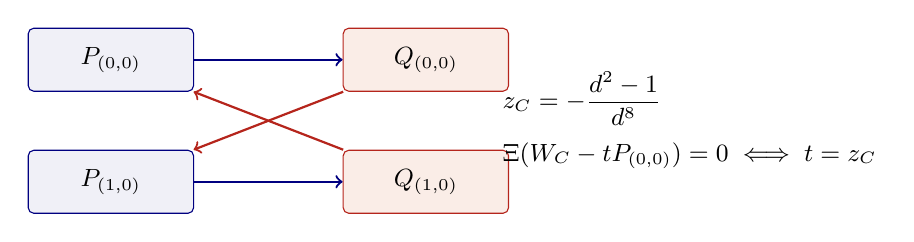
\begin{tikzpicture}[x=1cm,y=1cm,every node/.style={font=\small}]
\tikzset{pr/.style={draw=NavyBlue,fill=NavyBlue!6,rounded corners=2pt,minimum width=21mm,minimum height=8mm},
qr/.style={draw=BrickRed,fill=BrickRed!6,rounded corners=2pt,minimum width=21mm,minimum height=8mm}}
\node[pr] (p0) at (0,1.55) {\(P_{(0,0)}\)};
\node[pr] (p1) at (0,0) {\(P_{(1,0)}\)};
\node[qr] (q0) at (4,1.55) {\(Q_{(0,0)}\)};
\node[qr] (q1) at (4,0) {\(Q_{(1,0)}\)};
\draw[->,thick,NavyBlue] (p0) -- (q0);
\draw[->,thick,BrickRed] (q0) -- (p1);
\draw[->,thick,NavyBlue] (p1) -- (q1);
\draw[->,thick,BrickRed] (q1) -- (p0);
\node[anchor=west,align=left] at (4.85,0.78) {\(\displaystyle z_C=-\frac{d^2-1}{d^8}\)\\[5pt]\(\Xi(W_C-tP_{(0,0)})=0\iff t=z_C\)};
\end{tikzpicture}
\caption{The signed test is an ordered sewing of two distinct annular projectors at a time. The graph depicts the order of factors in \eqref{eq:negative}, not an embedded spatial cut or a classical simultaneous charge sample.}
\label{fig:cycle}
\end{figure}

\subsection{Arbitrary multiplicities and several marked cuts}

Let \(P_1,\ldots,P_N\) now be any finite set of actual charge projectors on a \(D\)-dimensional physical state space, with \(D\ge1\). Their ranks can be greater than one. If \(W(P)\) is an ordered word, put
\[
 X_W=(W+W^*)/2,\qquad Y_W=(W-W^*)/(2i).
\]
Adjoints are orientation-reversed cylinder maps in the unitary theory, and the coherent linear combinations define Hermitian operators. For real \(t\), the rank defects of \(X_W-tI\) and \(Y_W-tI\) are their eigenvalue multiplicities. Thus the Euclidean prices of both pencils determine
\begin{equation}\label{eq:trace}
       \Tr W=\Tr X_W+i\,\Tr Y_W
\end{equation}
including for a nonnormal word. This is a finite family of pencils, each parameterized by the exact real coefficient \(t\). It is not a claim that a bounded number of evaluations at predetermined \(t\)'s determines an arbitrary real spectrum.

\begin{theorem}[Finite simultaneous reconstruction]\label{thm:general}
The physical dimension and the price pencils of \(X_W-tI\) and \(Y_W-tI\) for words of length at most \(2D^2-1\) determine the simultaneous unitary class of the labeled projector family. For two complete sets of mutually orthogonal projectors the relative change of cut is therefore determined up to independent unitary bases in the two families' channel blocks.
\end{theorem}

\begin{proof}
The dimension is read from \(\mathsf f_L(I)\). Suppose another \(D\)-dimensional family \(\widetilde P\) gives the same price data. By \eqref{eq:trace} the traces of the indicated words agree. Let \(E_l\subset M_D(\FF)\oplus M_D(\FF)\) be the span of evaluation pairs \((W(P),W(\widetilde P))\) for words of length at most \(l\), including the identity. If \(E_l=E_{l+1}\), closure under left multiplication by each generator pair shows that \(E_l\) contains all longer words. As \(E_0\) has dimension one and the pair algebra has dimension at most \(2D^2\), \(E_{2D^2-1}\) contains the generated algebra. Hence the difference of traces vanishes on every word pair.

The generators are Hermitian, so for every noncommutative polynomial \(R\), the traces of \(R(P)^*R(P)\) and \(R(\widetilde P)^*R(\widetilde P)\) agree. Positivity implies \(R(P)=0\) if and only if \(R(\widetilde P)=0\). Thus evaluation gives a trace-preserving \(*\)-isomorphism between the concrete finite-dimensional \(C^*\)-algebras generated on the two spaces. For each simple block \(M_e(\FF)\) its central identity has trace \(e\) times its Hilbert-space multiplicity. The trace-preserving isomorphism therefore preserves all representation multiplicities and is implemented by a unitary. The converse is immediate. For two complete decompositions, choosing a unitary frame in each projector range gives the relative recoupling matrix, and the remaining choices are precisely the independent block-unitary gauges.
\end{proof}

The trace-word step is a finite-dimensional separation argument of the standard type studied in matrix invariant theory \cite{Procesi}. Its use here is to turn rank pencils into cut information even when there are internal multiplicities. This theorem does not simultaneously fix all three-valent fusion-vertex gauges across all external labels, and does not reconstruct ribbon operators that were not represented by the marked cuts.

\section{A native joint-Wilson test of the marked torus character variety}
\label{sec:torus-joint-wilson}

The preceding cut tests recover finite gluing data from which compatible
prices are computed.  Here we use a different, joint spectral test to
recover a classical configuration space.  No classical holonomy is used
to place the tensor indices. The two sites are incoming and outgoing copies of the torus,
placed at two fixed receiver sites with unit separation. The geometric input
is the standard interpretation of \(\mathrm{SU}(2)\) Wilson loops as
holonomy traces, not a prescribed metric on their spectrum.

\subsection{The physical operators and the twist convention}

Let \(r=k+2\) and \(\zeta_r=e^{\pi i/r}\).  The chiral
\(\mathrm{SU}(2)_k\) torus Hilbert space has orthonormal charge basis
\(e_n\), \(n=1,\ldots,r-1\), where \(n=2j+1\).
Turaev--Viro theory for the unitary modular category is the doubled
theory, so these chiral operators act on one factor of the physical
torus Hilbert space \(\mathcal H_k\otimes\overline{\mathcal H_k}\)
\cite{BalsamIII}.  In the positive fundamental-trace convention, the
marked meridian and longitude operators are
\begin{equation}
 D_r e_n=2\cos(\pi n/r)e_n,\qquad
 B_r e_n=e_{n-1}+e_{n+1},\qquad e_0=e_r=0.
 \label{eq:tw-torus-basic-operators}
\end{equation}
The first is the fundamental \(S\)-matrix quotient
\(S_{2n}/S_{1n}\); the second is fusion by the fundamental object.
The oriented meridional Dehn twist \(T_r\) multiplies \(e_n\) by
\(\exp\!\big(i\pi(n^2-1)/(2r)\big)\), up to one common framing phase.
The common phase cancels in the slope operator \(C_r=T_rB_rT_r^*\);
hence
\begin{equation}
 C_r e_n=\zeta_r^{\,n+1/2}e_{n+1}
          +\zeta_r^{\,-n+1/2}e_{n-1}.
 \label{eq:tw-torus-twist-operator}
\end{equation}
We fix the marking so that the slope of \(C_r\) is the product
of the two marked cycles.  Reversing the twist and the corresponding
marking just replaces the second classical eigenangle by its negative.

For clarity, these operators can be realized in the odd subspace of
\(\mathbb C[\mathbb Z/(2r)]\), with odd basis
\((\delta_n-\delta_{-n})/\sqrt2\),
\(n=1,\ldots,r-1\).  On the ambient space define
\[
 U_r\delta_n=\zeta_r^n\delta_n,\qquad
 V_r\delta_n=\delta_{n+1},\qquad J_r\delta_n=\delta_{-n}.
\]
They obey \(U_r V_r=\zeta_r V_r U_r\).  The restrictions of
\[
 U_r+U_r^*,\qquad V_r+V_r^*,\qquad
 \zeta_r^{-1/2}(U_r V_r+U_r^{-1}V_r^{-1})
\]
to the odd subspace are exactly \(D_r,B_r,C_r\).
In particular, the last formula is selfadjoint with the displayed
phase.  This is the standard torus skein representation
\cite{FrohmanGelca,CharlesMarche}.  Its product-to-sum identity follows
directly from the Weyl relation: if \(W_{(a,b)}=\zeta_r^{-ab/2}U_r^aV_r^b\)
and \(L_{\nu}=W_\nu+W_{-\nu}\), then
\begin{equation}
 L_\nu L_\mu
   =\zeta_r^{\,\det(\nu,\mu)/2}L_{\nu+\mu}
     +\zeta_r^{-\det(\nu,\mu)/2}L_{\nu-\mu}.
 \label{eq:tw-torus-product-sum}
\end{equation}
The physical three operators are the slopes \((1,0)\), \((0,1)\), and
\((1,1)\).  No commutativity at a finite level is assumed.

\subsection{A joint rank support theorem}

For a trial triple \(p=(p_1,p_2,p_3)\in\mathbb R^3\) and
a tolerance \(\delta>0\) define the positive operator and its spectral
projector
\begin{equation}
 K_{r,p}=(D_r-p_1I)^2+(B_r-p_2I)^2+(C_r-p_3I)^2,\qquad
 E_{r,p,\delta}=\boldsymbol{1}_{[0,\delta^2]}(K_{r,p}).
 \label{eq:tw-torus-joint-penalty}
\end{equation}
This is one gauge-invariant quantum spectral projection, not a product
of incompatible sharp projections.  In a unit vector, the expectation
of \(K_{r,p}\) is the sum of the squared errors of the three Wilson
operators.  The ordinary tensor of \(E_{r,p,\delta}\) across the two
marked torus ports has native two-site price \(\log_2 \operatorname{rank} E_{r,p,\delta}\)
when nonzero, and has zero spectral value when it vanishes
\cite{OpenAIPrice}.  An independent change of the positive port
separation multiplies a finite logarithmic price and does not change the
rank test.  The following statements concern this specified projector,
not the ranks of the three unsigned Wilson tensors by themselves.

\begin{theorem}[Joint-Wilson rank support and state count]
\label{thm:tw-torus-joint-wilson}
Let
\[
 X=\{(2\cos\alpha,2\cos\beta,2\cos(\alpha+\beta)):
                 (\alpha,\beta)\in(\mathbb R/2\pi\mathbb Z)^2\}.
\]
For each \(p\in X\) and each fixed \(\delta>0\), \(E_{r,p,\delta}\) has
positive rank for all sufficiently large \(r\).  For
\(p\notin X\) and \(0<\delta<\operatorname{dist}(p,X)\), it has zero rank
for all sufficiently large \(r\).  Moreover, with normalized torus Haar
measure \(d\mu\),
\begin{equation}
 \begin{aligned}
 \lim_{r\to\infty}\frac{\operatorname{rank}E_{r,p,\delta}}{r-1}
   &=\int_{(\mathbb R/2\pi\mathbb Z)^2}
     \boldsymbol{1}_{\{k_p(\alpha,\beta)\leq\delta^2\}}\,d\mu,\\
 k_p(\alpha,\beta)
   &=\big\|(2\cos\alpha,2\cos\beta,2\cos(\alpha+\beta))-p\big\|^2 .
 \end{aligned}
 \label{eq:tw-torus-count}
\end{equation}
Thus the eventually nonzero rank support at every positive tolerance
recovers \(X\), including its degenerate character points.  In the
doubled theory, using both chiral Wilson sets in the sum of penalties
gives \(X\times X\) and the analogous product-Haar count.
\end{theorem}

\begin{proof}
For spectral exclusion, work first in the full
\(\mathbb C[\mathbb Z/(2r)]\) representation.  In the quotient of bounded
matrix sequences by sequences tending to zero in operator norm, the
classes of \(U_r,V_r\) are commuting unitaries, since
\(\|U_rV_r-V_rU_r\|=|\zeta_r-1|\).
Continuous functional calculus then identifies the class of \(K_{r,p}\)
as the image of the continuous function \(k_p\) on the torus.  This
function is bounded below by \(\operatorname{dist}(p,X)^2\).
By continuity of the negative-part functional calculus, the negative
part of \(K_{r,p}-\operatorname{dist}(p,X)^2 I\) tends to zero in norm.
The same lower bound holds after restriction to the odd subspace.
This excludes sparse spectral outliers at any fixed positive distance,
a conclusion that would not follow from normalized traces alone.

For existence, every represented triple has a representative
\(\alpha\in[0,\pi]\) after joint angle inversion.  Let \(f\) be a nonzero
smooth bump of compact support in \((-1,1)\).  Choose the nearest integer
to \(r\alpha/\pi\) clipped to
\([\lfloor r^{2/3}\rfloor,r-\lfloor r^{2/3}\rfloor]\) as the charge
center \(c_r\), and let \(\sigma_r=r^{1/3}\).  In the physical odd
basis use the normalized vector
\[
 \psi_{r,n}=\mathrm{const}\cdot f\!\left(\frac{n-c_r}{\sigma_r}\right)
                 e^{-i\beta n}.
\]
The packet avoids both missing endpoints even at \(\alpha=0,\pi\).
On its support \(D_r\) differs from \(2\cos\alpha\) by
\(O(\sigma_r/r+|c_r/r-\alpha/\pi|)=O(r^{-1/3})\).
The normalized bump changes in \(\ell^2\) by \(O(\sigma_r^{-1})\)
under a unit shift, proving
\(\|(B_r-2\cos\beta)\psi_r\|=O(r^{-1/3})\).
The coefficients in \eqref{eq:tw-torus-twist-operator} applied to the
shifted packet differ from \(e^{\pm i\alpha}\) by \(O(r^{-1/3})\);
the phases of the shifted vector supply \(e^{\pm i\beta}\).
This gives
\(\|(C_r-2\cos(\alpha+\beta))\psi_r\|=O(r^{-1/3})\).
Hence \(\langle\psi_r,K_{r,p}\psi_r\rangle=O(r^{-2/3})\), and a
small eigenvalue exists below each fixed positive tolerance.

For the count, the full trace of a fixed \(U_r^aV_r^b\) vanishes for
all large \(r\) unless \(a=b=0\).  Its trace after multiplication
by \(J_r\) has absolute value at most two: a contributing basis vector
must solve \(2n\equiv-b\pmod{2r}\).  Insert \((I-J_r)/2\) when taking
the trace of a polynomial in \(D_r,B_r,C_r\).
Such a polynomial expands as a finite sum of Fourier monomials,
and commuting full \(U_r,V_r\) changes phases only by factors tending
to one.  The physical trace normalized by \(r-1\) therefore converges
to the torus Haar trace on every fixed polynomial in the classical
symbols.  Since the spectra of \(K_{r,p}\) lie in a fixed compact
interval, polynomial approximation gives weak convergence of its
empirical eigenvalue law.  The use of a discontinuous indicator in
\eqref{eq:tw-torus-count} is then legitimate: each level set of
\(k_p\) has Haar measure zero, because it is a nonconstant real-analytic
trigonometric polynomial (the term \(2\cos(2\alpha)\) from the first
square has no other term of that frequency to cancel it).
For the doubled model the two operators act on separate factors,
normalized traces factorize, and the penalty symbol is the sum of
the two classical penalties.  The endpoint construction, lower bound,
and continuity of the count apply to this sum as well.
\end{proof}

\subsection{Identification and scope}

The known flat character space for the marked torus consists of
commuting pairs in \(\mathrm{SU}(2)\) up to simultaneous conjugation.
They can be simultaneously diagonalized, with eigenangles up to joint
inversion.  Their trace triples satisfy
\[
 x^2+y^2+z^2-xyz=4,\qquad |x|,|y|,|z|\leq2.
\]
Conversely the two roots of this relation in \(z\) are
\((xy\pm\sqrt{(4-x^2)(4-y^2)})/2\), exactly the two relative-angle
choices.  For interior \(x,y\), \(z\) distinguishes the choices
since \(\sin\alpha\sin\beta\ne0\).  If either holonomy is central,
joint inversion identifies the would-be remaining ambiguity.
Thus the triple recovers the marked compact character variety everywhere.
The character variety and its quantum torus algebra are classical
ingredients; the new statement here is their recovery from the support
and state counts of the native rank probes
\eqref{eq:tw-torus-joint-penalty}--\eqref{eq:tw-torus-count}.
This is the space of allowed marked flat data, not a construction of
a nondegenerate metric from every flat pair, not an inferred curvature
radius, and not a dynamical selection of one state.



\section{Scope and conclusion}\label{sec:conclusion}

Physical cylinders and their marked operator compositions supply ordinary tensors whose Euclidean prices retain gluing data after the physical quotient. The joint torus Wilson test uses that same price on one spectral projector of a sum of squared constraints. It recovers the classical flat-character support and Haar count without assuming that the individual finite-level operators commute. The dimension construction measures a logarithmic growth law and an associative trace law. The coherent-pencil construction retains additional, signed cut information. Its extra operation is the coherent comparison to a prescribed projector or identity. Without that comparison, scalar multiplication leaves Choi rank unchanged, and knowing only the ranks of separated filters and sewings cannot recover their phases. The entire construction is invariant under triangulation changes and changes of coordinates that keep the specified physical insertions fixed. Prescribing a different set of physical marks or a different comparison operation defines a different test.

The model is the compact unitary TV theory. We do not derive its fusion category from the existence of an asymptotic spectral point, identify the receiver distance with a gravitational proper distance, or infer Lorentzian field dynamics. Nor do we use four-dimensional EPRL simplicity, opposite-parity Wilson transfer, or closed-manifold surgery. The finite statements follow from actual cut Hilbert spaces and specified linear operations on them.

\paragraph{Reproducibility.}
The accompanying standard-library scripts implement exact checks of the first finite fusion wall, diagonal-seed closure, level-two cut fractions, and the signed level-two projector composition. A separate exact phase-exponent replay checks the finite Weyl and odd-subspace conventions on the torus. The general statements and the torus limit are proved in the text.

\clearpage
\paragraph{Manuscript provenance.}
This is an AI-led research manuscript. The derivations and companion computations were checked internally; no external human expert review is claimed.

\begin{thebibliography}{99}
\bibitem{OpenAIPrice}
OpenAI, \emph{Euclidean geometry in the asymptotic spectrum of tensors}, preprint (2026).
\href{https://mathcommunity.github.io/oai-math-revised/papers/Euclidean-geometry-in-the-asymptotic-spectrum-of-tensors-November-24-2026/paper.pdf}{Preprint PDF}.

\bibitem{TuraevViro}
V.~G. Turaev and O.~Y. Viro, \emph{State sum invariants of 3-manifolds and quantum \(6j\)-symbols}, Topology \textbf{31}, 865--902 (1992).
\href{https://doi.org/10.1016/0040-9383(92)90015-A}{DOI}.

\bibitem{BalsamKirillov}
B. Balsam and A. Kirillov Jr., \emph{Turaev--Viro invariants as an extended TQFT}, \href{https://arxiv.org/abs/1004.1533}{arXiv:1004.1533} (2010).

\bibitem{BalsamII}
B. Balsam, \emph{Turaev--Viro invariants as an extended TQFT II}, \href{https://arxiv.org/abs/1010.1222}{arXiv:1010.1222} (2010).

\bibitem{BalsamIII}
B. Balsam, \emph{Turaev--Viro invariants as an extended TQFT III}, \href{https://arxiv.org/abs/1012.0560}{arXiv:1012.0560} (2010).

\bibitem{MugerDouble}
M. M\"uger, \emph{From subfactors to categories and topology II. The quantum double of tensor categories and subfactors}, J. Pure Appl. Algebra \textbf{180}, 159--219 (2003).
\href{https://arxiv.org/abs/math/0111205}{arXiv:math/0111205}.

\bibitem{Muger}
M. M\"uger, \emph{On the structure of modular categories}, Proc. Lond. Math. Soc. \textbf{87}, 291--308 (2003).
\href{https://arxiv.org/abs/math/0201017}{arXiv:math/0201017}.

\bibitem{MizoguchiTada}
S. Mizoguchi and T. Tada, \emph{Three-dimensional gravity from the Turaev--Viro invariant}, Phys. Rev. Lett. \textbf{68}, 1795--1798 (1992).
\href{https://doi.org/10.1103/PhysRevLett.68.1795}{DOI}.

\bibitem{EtingofNikshychOstrik}
P. Etingof, D. Nikshych and V. Ostrik, \emph{On fusion categories}, Ann. Math. \textbf{162}, 581--642 (2005).
\href{https://doi.org/10.4007/annals.2005.162.581}{DOI}.

\bibitem{KauffmanLins}
L.~H. Kauffman and S.~L. Lins, \emph{Temperley--Lieb Recoupling Theory and Invariants of 3-Manifolds}, Princeton University Press (1994).
\href{https://press.princeton.edu/books/paperback/9780691036403/temperley-lieb-recoupling-theory-and-invariants-of-3-manifolds}{Publisher}.

\bibitem{Procesi}
C. Procesi, \emph{The invariant theory of \(n\times n\) matrices}, Adv. Math. \textbf{19}, 306--381 (1976).
\href{https://doi.org/10.1016/0001-8708(76)90027-X}{DOI}.

\bibitem{FrohmanGelca}
C. Frohman and R. Gelca, \emph{Skein modules and the noncommutative torus},
Trans. Amer. Math. Soc. \textbf{352}, 4877--4888 (2000).
\href{https://arxiv.org/abs/math/9806107}{arXiv:math/9806107}.

\bibitem{CharlesMarche}
L. Charles and J. March\'e, \emph{Knot state asymptotics I: AJ conjecture and Abelian representations},
Publ. Math. IH\'ES \textbf{121}, 279--322 (2015).
\href{https://numdam.org/articles/10.1007/s10240-015-0068-y/}{Article}.

\end{thebibliography}
\end{document}
